\documentclass[10pt]{article}

\usepackage[a4paper, left=2cm, right=2cm]{geometry} % A4 paper size and thin margins

\usepackage{xcolor} % Required for specifying custom colours
\definecolor{grey}{rgb}{0.9,0.9,0.9} % Colour of the box surrounding the title

\usepackage{graphicx}
\usepackage[colorlinks=true, allcolors=black]{hyperref}
\usepackage{amsmath}
\usepackage{indentfirst}
\setlength{\parindent}{2em}

\usepackage[utf8]{inputenc} % Required for inputting international characters
\usepackage[T1]{fontenc} % Output font encoding for international characters
\usepackage[sfdefault]{ClearSans} % Use the Clear Sans font (sans serif)
%\usepackage{XCharter} % Use the XCharter font (serif)
\usepackage{float}

\newcommand{\tabincell}[2]{\begin{tabular}{@{}#1@{}}#2\end{tabular}} 	

\begin{document}
%----------------------------------------------------------------------------------------
%	TITLE PAGE
%----------------------------------------------------------------------------------------

\begin{titlepage} % Suppresses displaying the page number on the title page and the subsequent page counts as page 1
	
	%------------------------------------------------
	%	Grey title box
	%------------------------------------------------
	
	\colorbox{grey}{
		\parbox[t]{1.1\textwidth}{ % Outer full width box
			\parbox[t]{1.02\textwidth}{ % Inner box for inner right text margin
				\raggedleft % Right align the text
				\fontsize{34pt}{40pt}\selectfont % Title font size, the first argument is the font size and the second is the line spacing, adjust depending on title length
				\vspace{0.7cm} % Space between the start of the title and the top of the grey box
				
				< Journey Assistant >\\
                Software Requirement Specification\\
                Version 2.0\\
				
				\vspace{0.7cm} % Space between the end of the title and the bottom of the grey box
			}
		}
	}
	
	\vfill % Space between the title box and author information
	
	%------------------------------------------------
	%	Author name and information
	%------------------------------------------------
	
	\parbox[t]{1\textwidth}{ % Box to inset this section slightly
		\raggedleft % Right align the text
		\large % Increase the font size
		{\Large Group Member}\\[4pt] % Extra space after name
        Yiwen Song\\
        Zhihui Xie\\
        Weizhe Wang\\
        Huangfei Jiang\\
        Haoping Chen\\
		% Institution Name\\[4pt] % Extra space before URL
		% \texttt{LaTeXTemplates.com}\\
		
		\hfill\rule{0.2\linewidth}{1pt}% Horizontal line, first argument width, second thickness
    }
    
	
\end{titlepage}

\newpage

\begin{center}
    {\LARGE Modification History}
    
    \begin{tabular}{|c|c|c|c|} 
        \hline 
        Date&Version&Description&Author\\
        \hline  
        2019-04-02&1.0&Finish the architecture of the document.&Huangfei Jiang \& Weizhe Wang\\
		\hline 
		2019-04-17&1.1&Complement the content of interface.&Weizhe Wang\\
		\hline
		2019-06-18&2.0&Modify some diagrams&Zhihui Xie\\
		\hline
		& & & \\
		\hline
    \end{tabular}    
\end{center}

\newpage

\tableofcontents
\newpage

\section{Intruduction}
\subsection{Purpose}
This is a requirement specification document. In this document, we will define most of the system requirement, so that all the develop team member can have a clear picture of the whole system. We define not only the functional requirement, but the non-functional requirement as well. This is the main document of this define phase, in this phase, we also have glossary document, use case specification document and we offer a prototype.

\subsection{Scope}
This document is applied to our Journey Assistant System. It is a specialized document for our product.

\subsection{Definition}

\begin{table}[htb]
	\centering
	\begin{tabular}{|c|c|c|}
		\hline 
		Abbreviation&Term&Implication\\
		\hline  
		JAS&Journey Assistant System&Our Proposed System\\
		\hline 
		&Functional&Some requirement that need to be realized\\
		\hline
		&Non-functional&\tabincell{c}{Some requirement that can not be \\ realized but is indispensable to our system}\\
		\hline
		GAN&Generative Adversarial Network&\\
		\hline
		API&Application Program Interface&\tabincell{c}{A set of subroutine definitions, communication \\ protocols, and tools for building software.}\\
		\hline
		UDP&User Datagram Protocol&\tabincell{c}{One of the core members of the Internet protocol suite.}\\
		\hline
	\end{tabular}    

	\caption{Terms or Abbreviations}\label{Terms or Abbreviations}
\end{table}

	\subsection{Bibliography}
	\begin{itemize}
		\item[1.] <Object Oriented Software Engineering (Version 3)> (Tsinghua University Press)
		\item[2.] <Object Oriented Software Engineering Practice Guidelines> 
	\end{itemize}

\subsection{Sketch}
In this document, we are going to make some detailed descriptions on system requirements and related models and recount them by the order of function.

\section{System Overview}
Nowadays, people’s life has become better and better because of the reform and opening-up policy. More and more people decide to take a trip instead of staying at home during the holidays. However, since the destination is new to them, people usually can’t come up with a nice itinerary, which will influence their journey experience greatly. In the past time, people always search for different kinds of strategies and then knock them together. On the other hand, people who are busy studying and working may not have so much time to have a dreamful trip. With great pressure surrounding, a desired trip is unavailable to them.

Therefore, a network-based journey assistant system JAS is being called out. The traveler can plan their trip with this system handily, and of course get the help anytime they want. Our application will provide user with a platform which can assist them to draw up a perfect itinerary. Additionally, the platform is both professional and entertaining. With this application, user can not only get a detailed and highly-recommended journey itinerary but also have a virtual journey and feedback as they want. It will help people to fulfill their travel experience. 

We have following functions. 

\paragraph{\underline{Make an Itinerary on City}} After user’s selecting a certain city, system will produce a travel Itinerary according to user’s different requirements.

\paragraph{\underline{Customize a Trip}} Users can select scenic spots one by one, then system will let the users customize a trip and give user a fact-based experience feedback.

\paragraph{\underline{Give a Report}} Users can report the opinions about our system or their usage experience to us by our reporting interface.

\paragraph{\underline{Other Non-functional Requirement}}
\begin{itemize}
	\item[1.] The data of users should be protected against vicious hacking.
	\item[2.]	Customization information should be close to fact as much as possible.
	\item[3.]	Normally, the response time of our system should not be longer than 30s.
	\item[4.]	The UI should be beautiful and activate user’s desire to have a trip.
	\item[5.]	Statistics must be made.
	
\end{itemize}

\section{Targer System}
\subsection{Sketch}
Our project includes functional requirements and non-functional requirements. Functional requirements can be summarized as making a itinerary and customization of tourism, while non-functional requirements consist of response time, security, apperance and so on.

\subsection{Functional Requirement}
JAS provides users a handy tool to organize and manage their journey according to their kinds of requirements. 

First of all, it can help normal users to know more about the destination, such as climate, traffic situation, civilization and so on. After knowing about different places, users will make their mind to choose one or more city as their destination. Then users will get into a filter interfaces. In this interface, users can add conditions as they like which will be used to filter the itineraries in our alternative set. For example, the number of travelers, whether they have a pet or not, the style they want, the budget and any other requirements. All these demands will be considered in our next itinerary recommending.

During selecting condition, in order to produce an accurate and practical itinerary, system will provide users with different choices instead of letting them enter demands arbitrarily.

In addition, JAS also offer a powerful tool to customize a real trip and give users a feedback about experience.

Sometime users may not have time to have a trip, however, they still want to get some experience. With our application, time and money will not be constraints to our users anymore.
They can go through their trip virtually, while our system can give them a real experience.

When users try to enjoy our customization service, they also need to select a city at first. After city is decided, users can begin to choose the scenic spots. Each choice will be sent to the backend. After a nice and related cartoon, system will give a real feedback about this travel experience. Of course, feedback won’t be the same all the time, since we add some related random incidents to it. For example, if you choose a college as your destination, you may have a special experience with cute cats living in it! About the feedback, we will provide three types: some sentences (more sentient), some words (more accurate) and GAN’s perspective (Generative Adversarial Network). 

As a wonderful application, the report of users can’t be ignored. With a report interface, we can learn about our drawbacks and advantages in time.

Report will be conveyed to us through backend. When users begin to write a report, there will be two main types to choose: about data and about usage experience. Different types of report will be sent to different developers. 

\subsection{Non-functional Requirement}
\begin{itemize}
	\item[1.]Special security should be taken because the data of users cannot be leaked.
	\item[2.] As a featured function, customization must be as real as possible, since this is why users choose our application.
	\item[3.]  Response time should be as short as possible and had better not be longer than 30s. A loading flash should be displayed when users are waiting.
	\item[4.] Some data of users should be accessed so that we can make a better and personal recommendation.
	\item[5.]Users interface should be attractive, some related information can be displayed at first.
\end{itemize}

\subsubsection{Availability}
\begin{itemize}
	\item[1.] Since our application is a handy application, there is no requirement for users themselves.
	\item[2.] Our application need to be updated periodically with normal network.
	\item[3.] Two huge database should be equipped.
	\item[4.] Network should keep normal when users use our function.
\end{itemize}

\subsubsection{Reliability}
\begin{itemize}
	\item[1.] The system will be closed if we need to update or repair it. As for the other time, users can have a nice experience as they want. 
	\item[2.]To keep our application advance with the times, we need to update our database per month. 
	\item[3.] The information should be real absolutely. Description and real experience should be corresponding. 
\end{itemize}

\subsubsection{Performance}
\begin{itemize}
	\item[1.] The system response time (response to users’ request from servers to clients) must less than 30 second, if the network state is normal.
	\item[2.] Our system can deal with 1000 cases simultaneously.
	\item[3.]  The capicity depends on our database and related arithmetic.
	\item[4.] If the network state is abnormal, we can only provide users with off-line mode. In this mode, users can still search for information about scenario from local database.
	\item[5.]To achieve short response time, we need to have a powerful CPU or server to compute rapidly. However, to users, a well network state is the most important.  
\end{itemize}

\subsubsection{Supportability}
\begin{itemize}
	\item[1.] Our code standard and name rule will obey international rule strictly.
	\item[2.]Only developer can visit our back-end directly. 
\end{itemize}

\subsubsection{Design Constraint}
\begin{itemize}
	\item[1.] progamming language:Java, python, html and php.
	\item[2.] Java for main code, html and php for front-end, python for arithmetic.

\end{itemize}

\subsubsection{Interface}
In this part, we are going to show some detailed of our interface.
\paragraph{\underline{User Interface}}
Our system is designed as an application on mobile phone. Therefore, the user interface is an Android App on mobile terminal. When we are developing the user interface, we will use flat design style, so that our application will have a simple and elegant interface.

\paragraph{\underline{Hardware Interface}}
Our system will have a C/S structure (Client/Server structure), so we need to provide harewares which can surf the internet and run the browers. In order to satisfy the requirement of speed and convenience, we need to apply mobile calculation. Therefore, a facility which can run Android operation system is necessary.

\paragraph{\underline{Software Interface}}
The software interfaces we need are:

\begin{itemize}
	\item[(1)] Baidu Map API
	\item[(2)]Meituan Remark API
	\item[(3)]MySQL Server
	\item[(4)]Android
	
\end{itemize}

\paragraph{\underline{Communication Interface}}
The communication protocols we are going to use are:

\begin{itemize}
	\item[(1)] TCP/IP protocol.
	\item[(2)] UDP protocol
	\item[(3)] HTTP protocol
	
\end{itemize}

\subsubsection{Law, Copyright and Other Notice}
\begin{itemize}
	\item[1.]This software is created by all us group members together. We, unlearninng group, reserve all the right for the final explanation.
	\item[2.] Journey Assistant is a temporary name for our app, if it causes trademark infringement, welcome contact with us.
	
\end{itemize}

\subsubsection{Applicable Standard}
\begin{itemize}
	\item[1.] We are decided to produce an andorid software, hence it should obey the standard of andorid.
	\item[2.] The main language of our app is Chinese, English version is to be determined.
	
\end{itemize}

\subsection{System Model}
This section express detail requirements with concepts, methods and model diagram in UML.

\subsubsection{Scenery}
In this section, a representative scenario is selected to describe each participant that initiates a use case. Follow the format below:

\paragraph{\underline{Scenery One}}
\subparagraph{Scenery name} We should select a Specific name for each scenery.
\subparagraph{Actor instance} The specific actor involved in the scenario
\subparagraph{Event flow} Follow the steps to list the detailed flow

\subsubsection{Use Case Mode}
The specific steps in this section are as follows:

\begin{itemize}
	\item[(a)] 	Participant
	
	\begin{center}
		\begin{tabular}{|c|c|}
			\hline 
			Participants Name&Explanation\\
			\hline
			User&The user who uses this software\\
			\hline 
		\end{tabular}    
		\end{center}
	
	\item[(b)] 	Use case

	\begin{center}
		\begin{tabular}{|c|c|c|}
			\hline 
			Login&Sub-function Level&For identity confirm.\\
			\hline
Select Destination&Sub-function Level&\tabincell{c}{For the software to find \\corresponding city information.}\\
			\hline
Itinerary
Recommendation&User Target Level&\tabincell{c}{In this section, user are recommended to several\\ packaged  itineraries and he can select one of them.}\\
			\hline
Customization&User Target Level&\\	
			\hline
Generation&User Target Level&\\
			\hline
Report&User Target Level&\\	
			\hline 
		\end{tabular}    
		\end{center}

		\item[(c)] Introduce each use case in detail.
		
		\paragraph{\underline{Login}}

		\subparagraph{Preconditions and Post Conditions}
		\begin{itemize}
			\item There is no preconditions for this use case.
			\item When the user's input has been identified, the system will offer the access to the services, and the use case is over.
		\end{itemize}

		\subparagraph{Basic Scenarios} 
		\begin{itemize}
			\item[1.] The user inputs his username and password, and submit them to the system.
		
			\item[2.] The system checks the validity of the input. If the username and the corresponding password can be found in the database, the system will give out the destination-selection panel.
		\end{itemize}

		\subparagraph{Exception or Branches}
		If the input is not valid by the validity check, the system will give out a warning and the user should try it again.

		\paragraph{\underline{Select Destination}}
		\subparagraph{Definition} This is the requirement description for the Select Destination use case. Select Destination use case is for everyone who wants to make their itinerary or customize their journeys. The user can only select destination cities from a list we give, which we have their information in our database. Input a city that is not recorded is not permitted.

		\subparagraph{Preconditions and Post Conditions}
		\begin{itemize}
			\item The user has successfully logged in to the system.
			\item After the user has selected a destination city, he (or she) can make itineraries in the city or customize their journeys.
		\end{itemize}

		\subparagraph{Basic Scenarios}
		\begin{itemize}
			\item[1.] The system displays a list of cities that are available.
			\item[2.] The user selects a city he/she wants to go.
		\end{itemize}

		\subparagraph{Exception or Branches}
		After the user select one city to go to ,he could then choose which way he wants to pick up his travel itinerary.

		\paragraph{\underline{Make an Itinerary}}
		\subparagraph{Definition}
		This is the requirement description for the 'Make an Itinerary' use case. 'Make an Itinerary' use case is for every user who wants the system to recommend an itinerary in a specific city. The system will recommend several itineraries for the user.

		\subparagraph{Preconditions and Post Conditions}
		\begin{itemize}
			\item The user has successfully logged in and selected the destination.
			\item The system provides the user with several recommended itineraries.
		\end{itemize}

		\subparagraph{Basic Scenarios}
		\begin{itemize}
			\item[1.] The user inputs his preference of the journey, including the rythm, cost, and number of persons.
			\item[2.]The system makes several itineraries according to the user's preference, by our recommendation algorithms.
			\item[3.]The user picks one of the itineraries and saves it in his account.
		
		\end{itemize}

		\subparagraph{Exception or Branches}
		If the user does not want any of the itinerary, he can click the "no wanted" button, and the system will recommend another itinerary for him.

		\paragraph{\underline{Customization}}
		\subparagraph{Definition}
		This is the use case of customization part, which is also the core part in our travel assistant. Users can choose scenic spot one by one on our customization map, according to the spots information we posted on it.

		\subparagraph{Preconditions and Post Conditions}
		\begin{itemize}
			\item \begin{itemize}
				\item[(a)] The user has decided which city he preferred to go to and has confirmed the arriving data.
				\item[(b)] A map with every attraction of this city should be available to the user.
				\item[(c)] Each attraction has detailed information on the basic introduction, recommended spending time, the specialty and others’ comments, etc. 
			\end{itemize}
			\item When the user finished the customization and clicked a “finished” button, this use case is over and will turn to the generation part.
		\end{itemize}

		\subparagraph{Basic Scenarios} 
		\begin{itemize}
			\item[1.]	User enter the customization interface.
			\item[2.]	User glance over all of the attractions on the customization map
			\item[3.]	Therefore,  can user choose the first attraction of the city on our customization map.
			\item[4.] The basic information of attractions nearby will be output automatically in the form of card.
			\item[5.]User could choose to select the nearby attraction or other attractions as he wanted to be the next station.
			\item[6.] Then user will repeat step d and e until he want to put an end on this journey.
			\item[7.]User click the “finished” button and finish this use case.
			
		\end{itemize}

		\paragraph{\underline{Report}}

		\subparagraph{Definition}
		This use case is to describe the report from the users who have finished their authentic journey and wanted to make a comments or post a score on this journey. And it also basically includes the ordinary usage of report, which includes delivering some suggestions on our software or making some complains on our service.

		\subparagraph{Preconditions and Post Conditions}
		\begin{itemize}
			\item The user must have finished their journey in real time. And they should have a general impression on each place they have been to. 
			\item No post condition.
		\end{itemize}

		\subparagraph{Basic Scenarios}
		\begin{itemize}
			\item[1.] User confirms the finish of the real time journey, which means that clicking the “Journal Finished” button on the travel post generated before the real time journey.
			\item[2.]User could make a score on this journey and have some general comments on it if he like.
			\item[3.]Then the scenic spots list will be automatically unfolded under the travel post.
			\item[4.]It is encouraged for user to leave a message on each of the spots, in order to have a conclusion to themselves as well as leaving some advices for other users.
			\item[5.]When user have finished this, validation box will be popped up and user could make a tick on the check box to decide whether others can see this journey.
			\item[6.]Therefore, the score it marked and comments they made will be uploaded.
			\item[7.]User could review their journey and others can find see it and give a like to it.
			
		 \end{itemize}
		 
		 \subparagraph{Exception Scenarios}
		 If user have something else to concern about or lose the patience during scoring. A message box would pop up to ask users whether to contain and upload these message which has been made or quit it.

		 \paragraph{\underline{Generation}}
		 \subparagraph{Definition}
		 This use case allows admin to confirm the final itinerary and share it with others. After the admin has chosen itineraries we suggested or customize by himself, he can generate a result in the form of lists or posters. Therefore, he could use it conveniently during the tour or share it with their companions or other friends before the tour.

		 \subparagraph{Preconditions and Post Conditions}
		 \begin{itemize}
			 \item \begin{itemize}
				 \item[(a)] The arriving date to the destination city, the schedule of all scenic spots including expected tour time and the time spent on road from one spots to another.
				 \item[(b)] All information of the scenic spots, including the basic introduction, recommended spending time, the specialty and others’ comments should be known. 
			 \end{itemize}

			 \item No post condition.
		 \end{itemize}

		 \subparagraph{Basic Scenarios}
		 \begin{itemize}
			 \item[1.] User enter to the Generation interface.
			 \item[2.]	A post will be generated.
			 \item[3.] User could click the “share” icon to share it with others (such as companion or other friends).
			 
			 \begin{figure}[H]
				 \centering
				 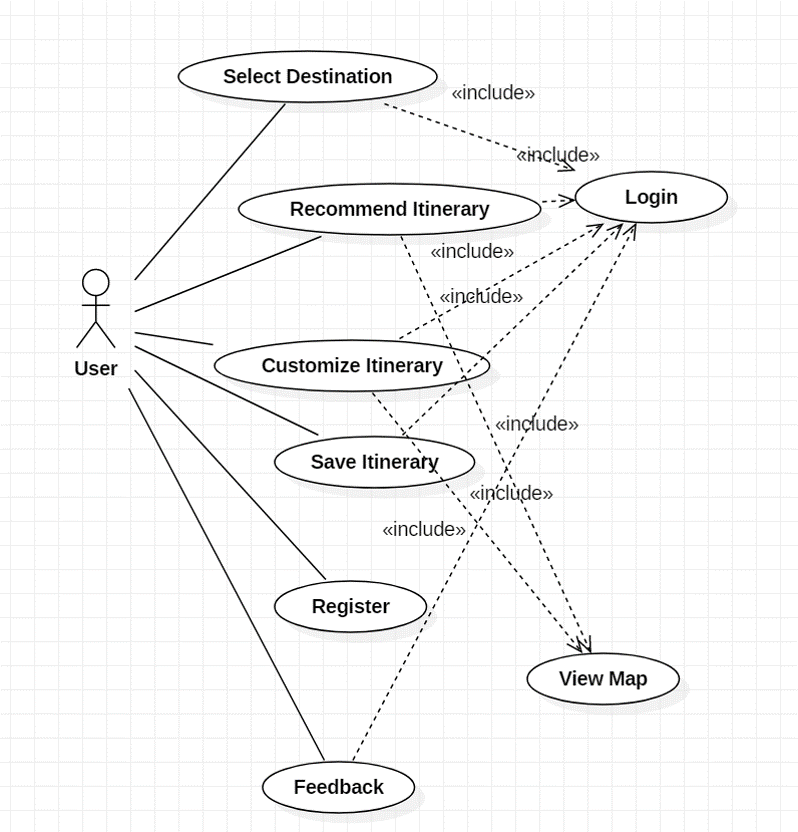
\includegraphics[width=14cm]{usecase.png} 
				 \caption{Use Case Diagram}
				 \label{Use Case Diagram}
			 \end{figure}
			 
			 
		 \end{itemize}
\end{itemize}

\subsubsection{Object Model}
The followings are some detailed introductions.

\begin{table}[htb]
	\centering
	\begin{tabular}{|c|c|c|c|}
		\hline 
		Entity class Name&Attributes&Association class&Definition\\
		\hline
		User&\tabincell{c}{Name:String\\
		Account:Interger\\
		Password:Integer}
		&\tabincell{c}{To Map: Select one city;\\
		To final itinerary: \\Confirm the schedule}&The user of JAS
		\\
		\hline
		Attraction&\tabincell{c}{Name:String\\
		Rank:Integer\\
		General Cost Time: Time\\
		General Cost Money:Integer}
		&None&Attractions available in map
		\\
		\hline 
		Map&\tabincell{c}{Name of city: String\\
		NumofAttr: integer\\
		Cost Time between \\attractions: List[integer]
		}
		&From User: Select one city&\tabincell{c}{The visualized map on \\which user could \\select attractions}
		\\
		\hline 
		Final itinerary&\tabincell{c}{Start time: Date\\
		Leave time: Date\\
		Buget:Interger\\
		City:String}
		&\tabincell{c}{From User: Confirm \\the schedule}&\tabincell{c}{List the schedule \\of this travel}
		\\
		\hline 
	\end{tabular} 

	\caption{Entity Class Definition Table}\label{Entity Class Definition Table}
\end{table}

\begin{table}[htb]
	\centering
	\begin{tabular}{|c|c|}
		\hline 
		Boundary class name&Definition\\
		\hline
menu&The menu which user could choose \\
		\hline

	\end{tabular} 

	\caption{Table Boundary Class Definition}\label{Table Boundary Class Definition}
\end{table}

\begin{figure}[H]
	\centering
	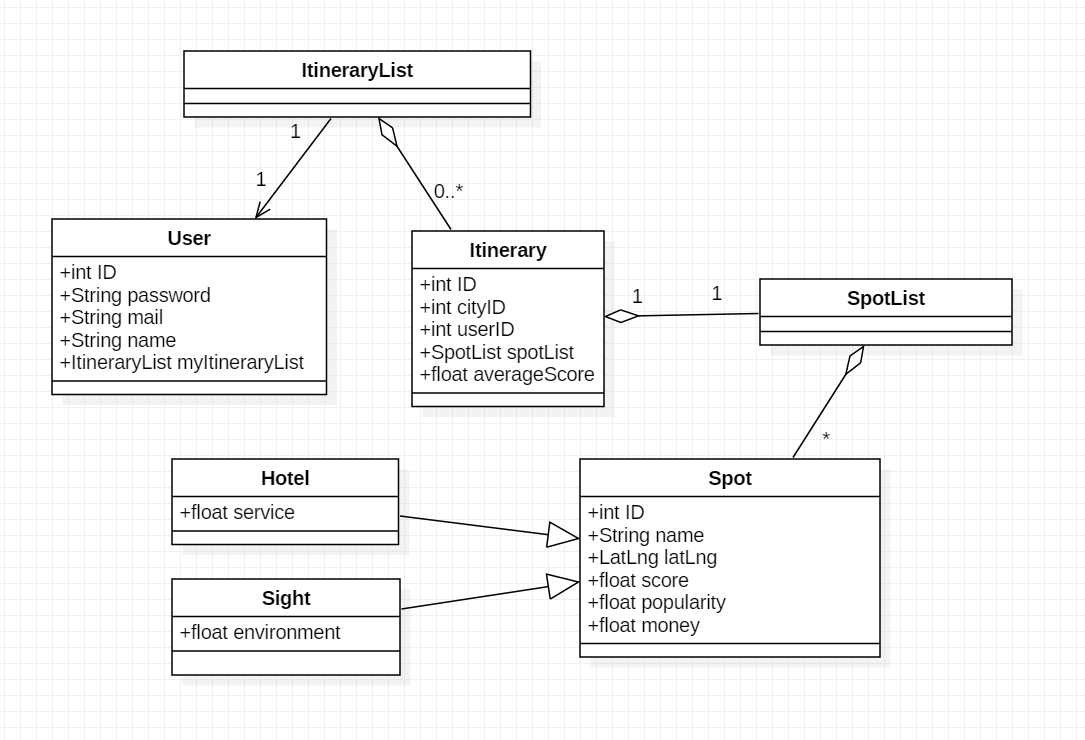
\includegraphics[width=14cm]{class.png} 
	\caption{Class Diagram}
	\label{Class Diagram}
\end{figure}

\subsubsection{Dynamic Model}
\begin{figure}[H]
	\centering
	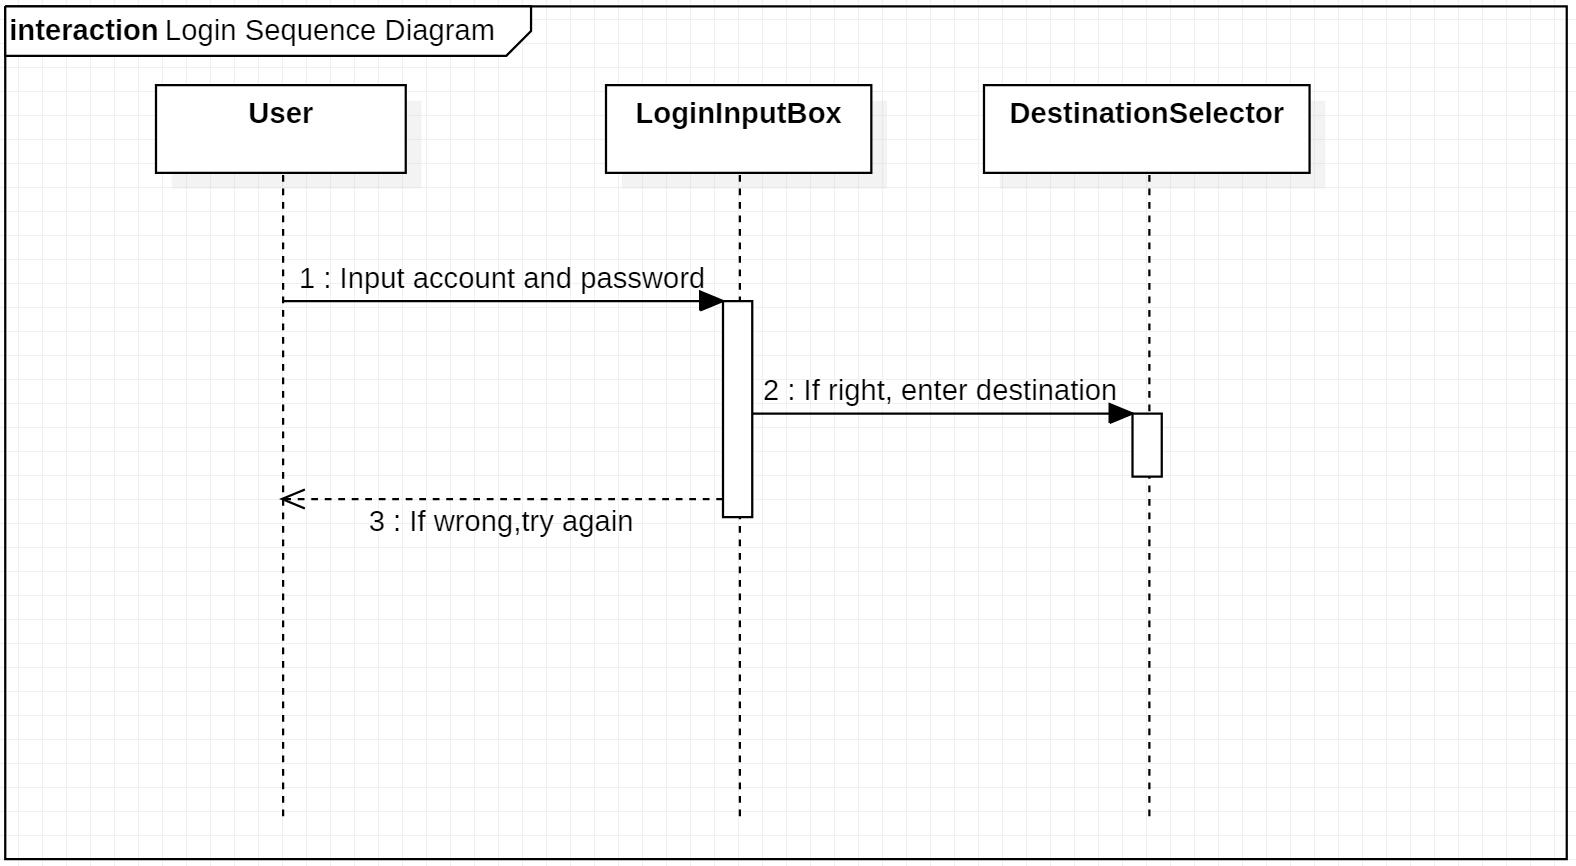
\includegraphics[width=14cm]{login.jpg} 
	\caption{Login Sequence Diagram}
	\label{Login Sequence Diagram}
\end{figure}

\begin{figure}[H]
	\centering
	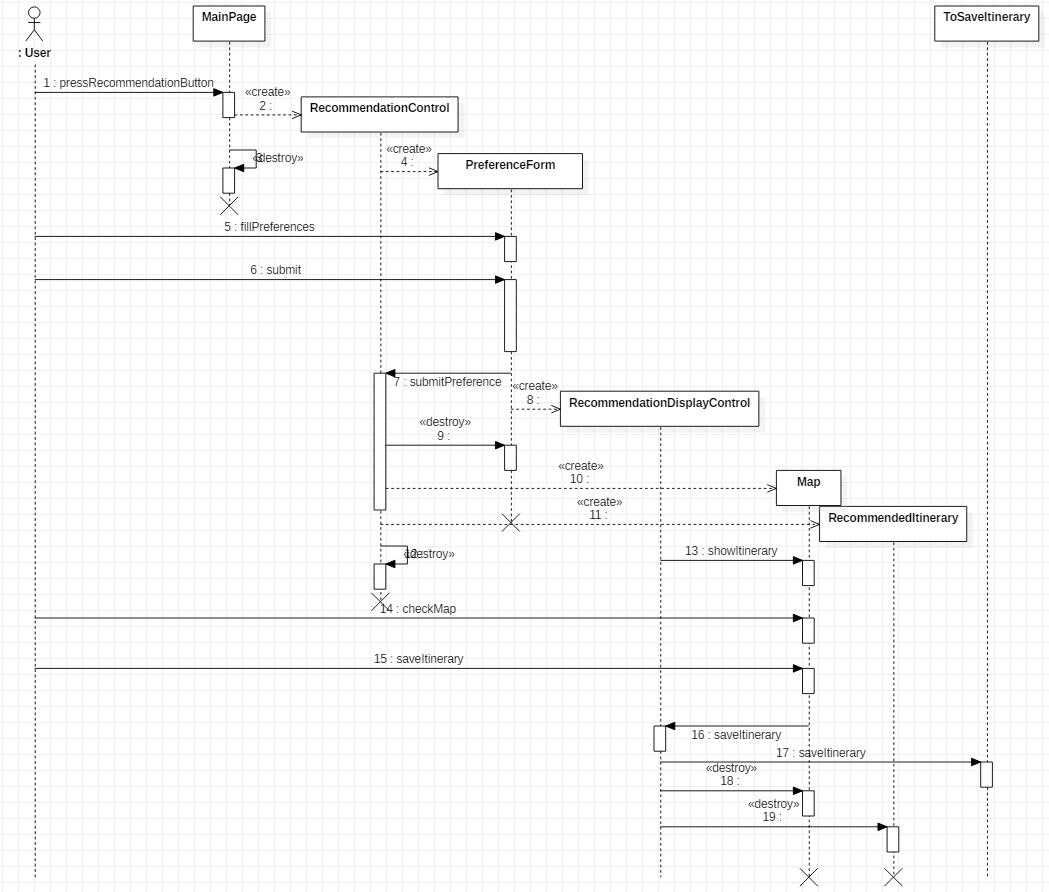
\includegraphics[width=14cm]{recommendation.png} 
	\caption{Recommendation Diagram}
	\label{Recommendation Sequence Diagram}
\end{figure}

\begin{figure}[H]
	\centering
	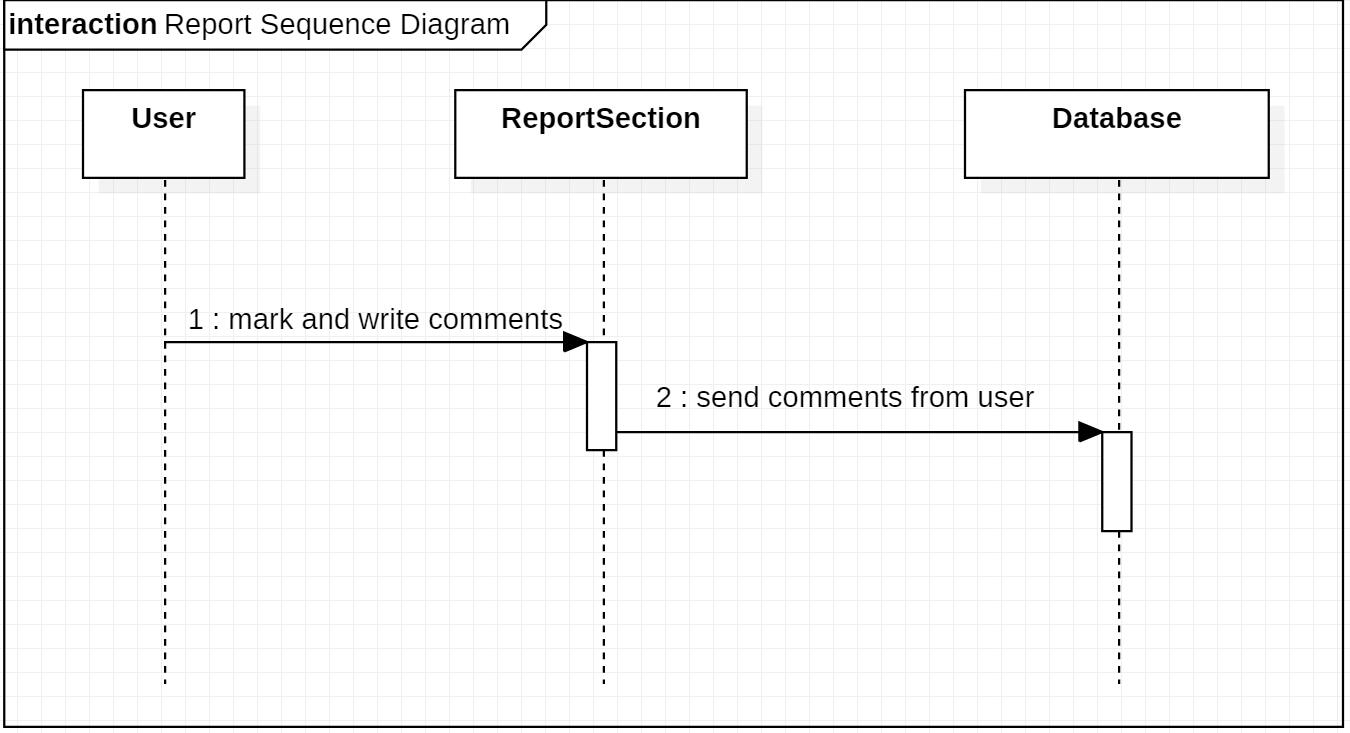
\includegraphics[width=14cm]{report.jpg} 
	\caption{Report Diagram}
	\label{Report Sequence Diagram}
\end{figure}

\begin{figure}[H]
	\centering
	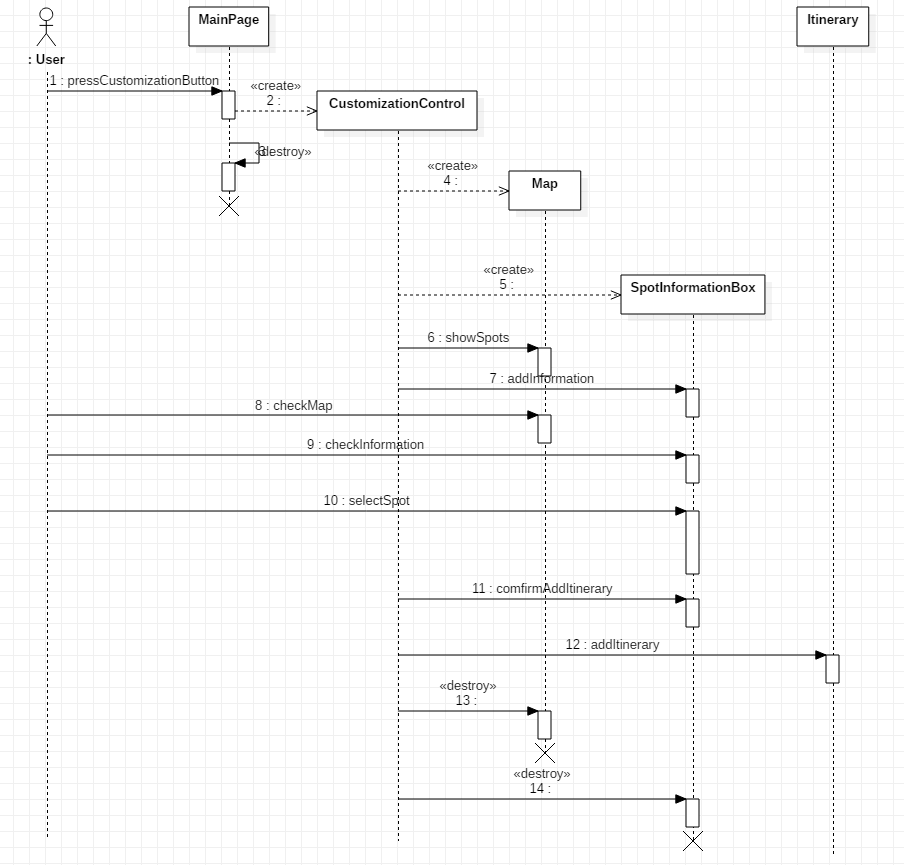
\includegraphics[width=14cm]{customization.png} 
	\caption{Customization Sequence Diagram}
	\label{Customization Sequence Diagram}
\end{figure}

\subsubsection{User Interface} 
According to our system’s function, the user interface should contain main page, log-in page, register page, itinerary-design page, customization page, personal page and so on. And there are some details about them:

\paragraph{\underline{Main Page}}
In our main page, there are name of our application, developer, password-retrieve button, log-in button and register button which can link to corresponding page. Also, some recommended news will be put on main page. Additionally, there are also four buttons which can link to itinerary-design page, customization page, report page and personal page respectively.

\paragraph{\underline{Log-in Page}}
This page is for users’ logging in, users should enter their username and password. User can also click on the register button which lay on the bottom of page to register in our application. If possible, we can allow user to log in with their QQ, Wechat or Alipay.

\paragraph{\underline{Register Page}}
In register page, there is a submit button and a table for user to enter their information, such as new username, password, phone number and verification code. At the bottom of this page, there are two buttons. One links to main page, and the other one links to log-in page.

\paragraph{\underline{Itinerary-Design Page}}
As one of our main function, itinerary design have its own page. In this page, there will be a detailed table and a submit button. In the table, user can select the origin, densitination as well as filtering conditons. After submitting the data, result will be display on this page and a return button is provided. Main page button also will be equipped.
e)	Customization page: Customization is our featured function. In this page, user should select the origin and densitination through a simple table firstly. Then, a map will be displayed on the page, and user can click on the map to begin customization. The feedback will be displayed after customizing.

\paragraph{\underline{Customization Page}}
Customization is our featured function. In this page, user should select the origin and densitination through a simple table firstly. Then, a map will be displayed on the page, and user can click on the map to begin customization. The feedback will be displayed after customizing.

\paragraph{\underline{Personal Page}}
In this page, people can check their selected itinerary and change their settings. In addition, a report button is equipped. Users are required to fill in a table and submit it to our system.
%----------------------------------------------------------------------------------------

\end{document}
